\documentclass[11pt,letterpaper]{article}
\usepackage[lmargin=1in,rmargin=1in,tmargin=1in,bmargin=1in]{geometry}
\usepackage{../style/homework}
\setbool{quotetype}{true} % True: Side; False: Under
\setbool{hideans}{true} % Student: True; Instructor: False

% -------------------
% Content
% -------------------
\begin{document}

\homework{1: Due 01/24}{When I was young I observed that nine out of every ten things I did were fails, so I did ten times more work.}{George Bernard Shaw}

% Problem 1
\problem{10} A certain subspecies of oak tree grows to an average height of 87~ft. After five years of growth, the growth rate of these oaks is approximately constant at a rate of 13~in per year. An ecologist finds the current height of an oak estimated to be 8~years in age to be 8~ft tall. Let $H(t)$ denote the height (in feet) of the tree $t$ years from its `birth.' 
	\begin{enumerate}[(a)]
	\item Explain why $H(t)$ is approximately linear. 
	\item Find $H(t)$ and sketch it in the plot below. 
	\item Interpret the slope of $H(t)$.
	\item Interpret the $y$-intercept for $H(t)$.
	\item Find approximately how many more years until the tree reaches its `adult height.' 
	\end{enumerate}
	
	\vfill
	
	\[
	\fbox{
	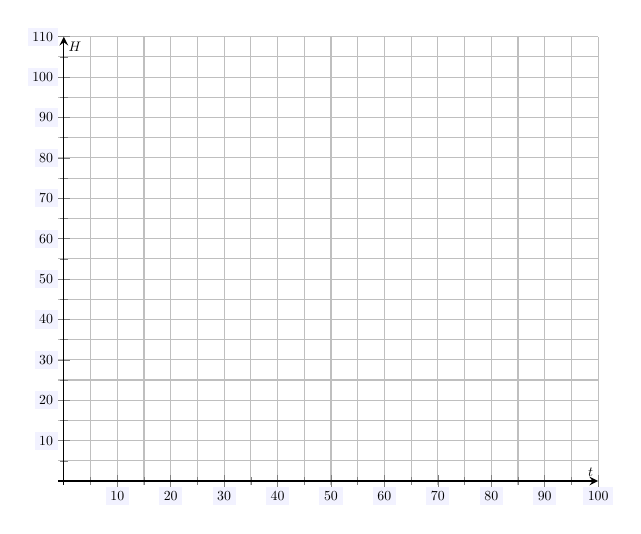
\begin{tikzpicture}[scale=1,every node/.style={scale=0.5}]
	\begin{axis}[
	grid=both,
	axis lines=middle,
	ticklabel style={fill=blue!5!white},
	xmin= -1, xmax=100,
	ymin= -1, ymax=110,
	xtick={0,10,...,100},
	ytick={0,10,...,110},
	minor x tick num = 1,
	minor y tick num = 1,
	xlabel=\(t\),ylabel=\(H\),
	]
	\end{axis}
	\end{tikzpicture}
	}
	\] 



\newpage



% Problem 2
\problem{10} Compute the following:
	\begin{enumerate}[(a)]
	\item 76\% of 8,571
	\item 16\% of 56.8
	\item 155\% of 11
	\item 78 decreased by 54\%
	\item 280 increased by 40\%
	\item 54 increased by 110\%
	\end{enumerate}
	
	

\newpage



% Problem 3
\problem{10} The economy in a certain nation is devolving into panic due to recent world events. Economists in the country are trying to keep track of the resulting inflation. A good which currently costs \$30 is estimated to increase in price by 8\% each month over the next 2 months. 
	\begin{enumerate}[(a)]
	\item How much will the good cost after the end of the two months? Be sure to justify your answer. 
	\item Is your answer in (a) the same as raising the original price by 16\%? Explain. 
	\item If the price simply increased to \$40, by what percentage did the price increase from the original price?
	\item If the inflation continues at this rate, how much will the good cost two years from now?	
	\end{enumerate}


\end{document}